\DocumentMetadata{}
\documentclass{scrartcl}

\usepackage{xcolor}
\usepackage{tcolorbox}
\usepackage{tikz}
\usetikzlibrary{positioning, shapes.geometric, arrows.meta}

\usepackage{titlesec}

\usepackage[skip=10pt, indent=0pt]{parskip}
\usepackage[backend=biber,style=authoryear]{biblatex}
\usepackage[top=20mm,bottom=20mm,left=20mm,right=20mm]{geometry}
\usepackage[colorlinks=true]{hyperref}
\addbibresource{ref.bib}



\titleformat{\section}{\normalfont\Large\bfseries}{{\color{purple}\S}}{0.5em}{}
\titleformat{\subsection}{\normalfont\bfseries}{{\color{purple}\S\S}}{0.5em}{}
\titleformat{\subsubsection}{\normalfont\small\bfseries}{{\color{purple}\S\S\S}}{0.5em}{}

\title{CS4920 | Essay 2 Final}
\author{Aayush Bajaj | z5362216}
\date{\today}


\begin{document}
\maketitle
\tableofcontents

\dotfill
\newpage
\section{Question 1}

\begin{tcolorbox}[colback=white,colframe=purple,sharp corners]
    What is the difference between \emph{explainability} and \emph{interpretability}? In what ways might XAI be helpful or unhelpful?
\end{tcolorbox}

\subsection{Response}

XAI is helpful in finance, health, transport, etc, but current XAI is not meeting the expectations because our approaches are too technical and not interdisciplinary enough (Malizia 2023).

XAI is only unhelpful in the sense that improving interpretability comes at the cost of accuracy (Lipton 2018). (Think decision trees vs. deep neural nets.)

Mariarosaria Taddeo affirms the importance of both explainability and interpretability in her 2022 paper, but positions interpretability as more important than explainability. She does this in her first principle (of 8) in designing (Non-Lethal) Automated Weapon Systems. She asserts that such systems should be more interpretable and less explainable.

Rosaria draws her definition of interpretability and explainability from Rudin's 2019 paper as intepretability being the designing of models whose operations are transparent and understandable to humans, whilst explainability is the ad-hoc attempt of making sense of opaque models after they have been trained (LIME, SHAP).

Finally, there is still a smudged view of both interpretability and explainability, where both are used (unfortunately) synonymously in the AI literature (Doshi-Velez and Kim). 

\newpage
\section{Question 2}
\begin{tcolorbox}[colback=white,colframe=purple, sharp corners]
    We can remove discrimination by removing all group membership information from the dataset (for example, by removing gender data), and the model would become fair to different gender groups. Similarly, we can remove information about age or race. Do you agree or disagree with this approach of \emph{fairness through unawareness?} Why?
\end{tcolorbox}

\subsection{Response}

This seems like it might work, but a paper by Cornacchia in 2023 disproved it by entertaining the counterfactual ``If gender information was removed, then what would happen?".

It turns out the algorithms just learn the same features in a different latent space through proxy variables.

Yates splits the biases into three buckets of algorithmic, activity and data. Clearly removing the data bias will not affect the systemic bias that also prejudices a group.

And finally, perhaps the most informative paper on the matter: The (Im)possibility of Fairness, Friedler et al. 2016 positions the worldview of being individually fair as mutually exclusive with being group-fair. The authors mathematically juxtapose the WYSIWYG (What You See is What You Get) data approach with the WAE (We are All Equal) approach.

Thus, whilst you can remove group discrimination by removing the group information, you will not eliminate ALL discrimination, and further there is still a large chance for the group relationships to be learned nonetheless.


\newpage
\section{Question 3}
\begin{tcolorbox}[colback=white,colframe=purple, sharp corners]
What does \emph{everyday leadership development} look like? Give an example (either actual or counterfactual) from your Group Project in terms of Positive Organisational Scholarship. In your answer, place yourself in the role of hypothetical Group Project Manager.
\end{tcolorbox}

\subsection{Response}
From the paper by Ashford and DeRue (2012), we learn that the Positive Organisational Scholarship perspective enables people to become leaders at all levels of an organisation, and that one needs to take responsibility for their own leadership development.

In the context of our Group Project I was cognisant of the Leadership lecture and of constructing a Mindful Engagement Feedback loop with both actual and counterfactual hypotheticals.

\begin{center}
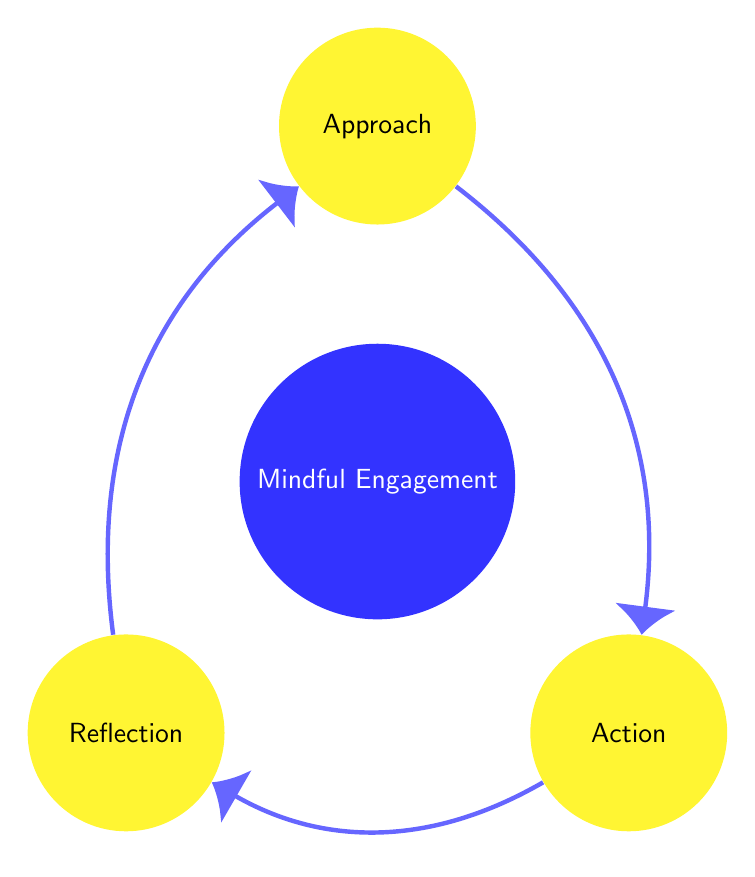
\begin{tikzpicture}[node distance=1.5cm, every node/.style={font=\sffamily}, 
    roundnode/.style={circle, draw=none, fill=yellow!80, minimum size=2.5cm},
    centralnode/.style={circle, draw=none, fill=blue!80, text=white, minimum size=3.5cm},
    arrow/.style={-{Latex[width=8mm]}, ultra thick, blue!60}]

    % Nodes
    \node[centralnode] (center) at (0,1) {Mindful Engagement};

    \node[roundnode] (approach) [above=of center] {Approach};
    \node[roundnode] (action) [below right=of center] {Action};
    \node[roundnode] (reflection) [below left=of center] {Reflection};

    % Curved Arrows
    \draw[arrow] (approach) to[bend left=30] (action);
    \draw[arrow] (action) to[bend left=30] (reflection);
    \draw[arrow] (reflection) to[bend left=30] (approach);

\end{tikzpicture}
\end{center}

One particular hypothetical was between myself and Shayyan wherein I suggested he do the fourth part of the assignment. I ran counterfactuals against Shayyan particularly because I did not want to overstep. In the end I maintained a forward but flexible stance on delegating parts, simply getting to know my Group Members and asking about their degrees / courses and interests so that I may act as the kintsugi of the group and lead by not leading (Lao Tzu, Tao Te Ching)

\newpage
\section{Question 4}
\begin{tcolorbox}[colback=white,colframe=purple, sharp corners]
    What is ethical principlism? Is it useful, dangerous or both? Why?
\end{tcolorbox}

\subsection{Response}
Ethical Principlism falls within Applied Ethics and is different to both Normative and Meta-ethics. As such, due to its closeness with the physical world, principlism becomes both useful and dangerous. I believe though, that the pros outweigh the cons.

The origins date back to Biomedical Ethics and Beauchamp and Childress' (2004) work on the matter. In a historical development paper by Beauchamp and DeGrazia, they recount that ``a single-principle theory has struck many as misguided as well as presumptous or dogmatic". Here, they are referring to Utilitarian and Deontological approaches. The authors then go on to highlight that adherents to most Normative Ethical camps ``agree at the level of the principles of biomedical ethics". As such Principlism was born.

Giving instruction to ``be alert to matters of justice", and ``to think about justice", suddenly ``action" became promoted to first-class citizen out of Normative Ethics.

Furthermore, any conversation of Justice alludes to Rawls. Indeed, his work on Reflective Equilibrium underpins what the Justice is interpretted as in the following 4 Principlism Principles:

\begin{enumerate}
    \item Respect for Autonomy
    \item Beneficence
    \item Non-maleficence
    \item Justice
\end{enumerate}

Finally, by considering a tangible example of Emergency Department Triaging, we can quickly see how Ethical Principle is more useful than dangerous.

\begin{enumerate}
    \item Listen to the patients
    \item Do good
    \item Do not cause harm
    \item Be fair
\end{enumerate}

Compare this now, to a Virtue Ethicist who would be forced to ask the ambiguous question:

What would an virtuous person do in this situation?

Overall, it is clear that Ethical Principlism is a set of percolated principles, informed by Normative and Metaethical study that can be used to derive ethical documents such as the ACM code.

As a concluding caveat Principlism is not perfect, and we shall see 2 arguments below that turn the simplicity of Principlism into its naivete.

+ Cybersecurity ethics. They just include Explicability. "A Principlist Framework for Cybersecurity". 2021 et al.

\newpage
\section{Question 5}
\begin{tcolorbox}[colback=white,colframe=purple, sharp corners]
    Why does Munn claim that AI Ethics principles are meaningless, isolated, and toothless? Is he correct? Why?
\end{tcolorbox}

\subsection{Response}
He is correct. There is a gap between high-minded principles (as enumerated in Q4) and technological practice. 

Meaningless means commendable values such as ``fairness" and ``privacy" break down when subjected to scrutiny. Value ``X" can really be bent to mean whatever you need it to mean, and furthermore developers may conduct an ``ethics shopping".

Isolated means that unethical AI is the logical byproduct of an unethical industry! Munn provides case studies of Silicon Valley which highlight the misogynistic environment and of Universities that fail to teach the appropriate macro-ethical concepts.

Toothless means that AI ethical principles have failed due to the lack of consequences. Munn provides a case study of Google here, who whilst producing an ethical board (great!), do not give the board any authority to enforce actions in any meaningful way (boo!).

Ultimately, despite the pessimism of Munn, he provides a solution in that AI Ethics should be rebranded to AI Justice.


\newpage
\section{Question 6}
\begin{tcolorbox}[colback=white,colframe=purple, sharp corners]
    What are the Menlo Principles? Which type of normative ethics might be used to justify each of the principles? Why?
\end{tcolorbox}

There are 4 Principles:
\begin{enumerate}
    \item Respect for persons \(\rightarrow\) Kantian
    \item Benificence \(\rightarrow\) Utilitarianism
    \item Justice \(\rightarrow\) Virtue Ethics
    \item Respect for Law \(\rightarrow\) Rule-based Utilitarianism
\end{enumerate}

It is worth noting the replacement of Respect for Law with Non-maleficence in the Principlism approach. The reason for this is that the Menlo Principles add legal and public accountability to their status quo.

The existence of the Menlo Principles as an entity proves what a study of all the Normative Ethics individually suggests: we need an ensemble of these models to make effective ethical decisions.

Briefly, I recount each of the stances and construct a mapping between their core values and the Menlo Principle in Question

\begin{enumerate}
    \item \textbf{Kant:} Autonomy and rational agency are central. The Categorical Imperative demands that we treat others as ends in themselves, never merely as means \(\rightarrow\) Respect for Persons.

    \item \textbf{Mill:} Right actions are those that promote the greatest happiness for the greatest number \(\rightarrow\) Beneficence reflects this utilitarian aim of maximizing overall good.

    \item \textbf{Aristotle:} Justice is a cardinal virtue and a mean between selfishness and selflessness. It sustains social harmony and reflects moral excellence \(\rightarrow\) Justice aligns with Virtue Ethics.

    \item \textbf{Rule Utilitarians:} Moral rules (like laws) help ensure consistent, beneficial outcomes for society over time \(\rightarrow\) Respect for Law ensures accountability through stable rule-following.
\end{enumerate}

\newpage
\section{Question 7}
\begin{tcolorbox}[colback=white,colframe=purple, sharp corners]
    Assume Nihilistic Error Theory. How might the moral education of computer science students then proceed?
\end{tcolorbox}

\subsection{Response}
Error Theory posits that the truth-maker is unknowable, and additionally nihilism posits that there is no way to know the truth-value of these moral judgements.

As such there are no moral facts, and morality is a systematic error rooted in false beliefs about objective value.

With this in mind, we must construct a moral education for computer science students without appealing to objective moral truths. 

Instead of collapsing into relativistic apathy or nihilistic despair, we can structure things much in the way that this course has done so:

\begin{itemize}
    \item normative ethics are socially and practically useful despite nihilistic error theory
    \item professional codes (acm, ieee) can be thought as shared fictions
    \item bias, fairness explored in terms of stakeholder values
    \item transparency, explainability focusses on pragmatic necessity instead of a moral imperative
    \item pragmatic pluralism, where metaethical consideration is given to competing ethical frameworks to enrich utility not truth
    \item systems thinking as opposed to individual blame
\end{itemize}

To summarise, even under nihilistic error theory, moral education in computer science can proceed constructively — not by asserting false objectivity, but by reframing ethics as a socially negotiated toolkit that enables cooperation within an otherwise amoral universe.


\newpage
\section{Question 8}
\begin{tcolorbox}[colback=white,colframe=purple, sharp corners]
    What are the risks and opportunities for our understanding and practice of moral responsibility given the rise of automated weapons systems in particular, and automated decision-making systems in general?
\end{tcolorbox}

\subsection{Response}
Moral Responsibility is defined and distinguished by Taddeo and Blanchard in \underline{A Moral Gambit}:
\begin{enumerate}
    \item Intentionality
    \item Causality
    \item Consequence
    \item Choice
\end{enumerate}

The authors distinguish this from meaningful moral responsibility, which can only apply to Non-Lethal Automated Weapon Systems, as deployment of Lethal Autonomous Weapon Systems is ``morally unacceptable".

Thus the risks posed by automated systems are manifold:

\begin{itemize}
    \item eroding choice as AWS / ADM are by definition automated
    \item unsatisfiability triad: ADM cannot simultaneously satisfy \emph{fairness, accountability and accuracy}. attempts to improve one (fairness) reduces the other (accuracy). this is bad because moral responsibility requires all three. this can also result in ethics-bashing (Bietti 2020)
    \item risk of moral deskilling and normative drift. over time, human capacity for complex decision making and ethical integrity could erode.
    \item opacity of ADM's allows institutions to exploit ethics-washing (Bietti 2020)
\end{itemize}

Yet, there are also opportunities:

\begin{itemize}
    \item HCAI with High Control and High Automation (Shneiderman 2020)
    \item IEEE couples individual and institutional responsibility with authors of ADM's
\end{itemize}

It seems that ultimately automated systems — especially in high-stakes domains like warfare or sentencing — have more cons than pros. The unsatisfiability of the fairness-accountability-transparency triad underscores the need for human oversight and Taddeo's Moral Gambit plus the IEEE supports the need for a HITL (Human in the Loop).

In conclusion, the risks outweigh the benefits and whilst we have systems in place to facilitate a constrained optimisation of this Wicked Problem, we are still stuck in a local minima for now.


\newpage
\section{References}

\nocite{*}
\printbibliography[heading=none]

\end{document}
